\section{Was ist Autonomes Fahren?}

\begin{frame}
    \frametitle{Was ist Autonomes Fahren?}

    \begin{figure}[H]
        \centering
        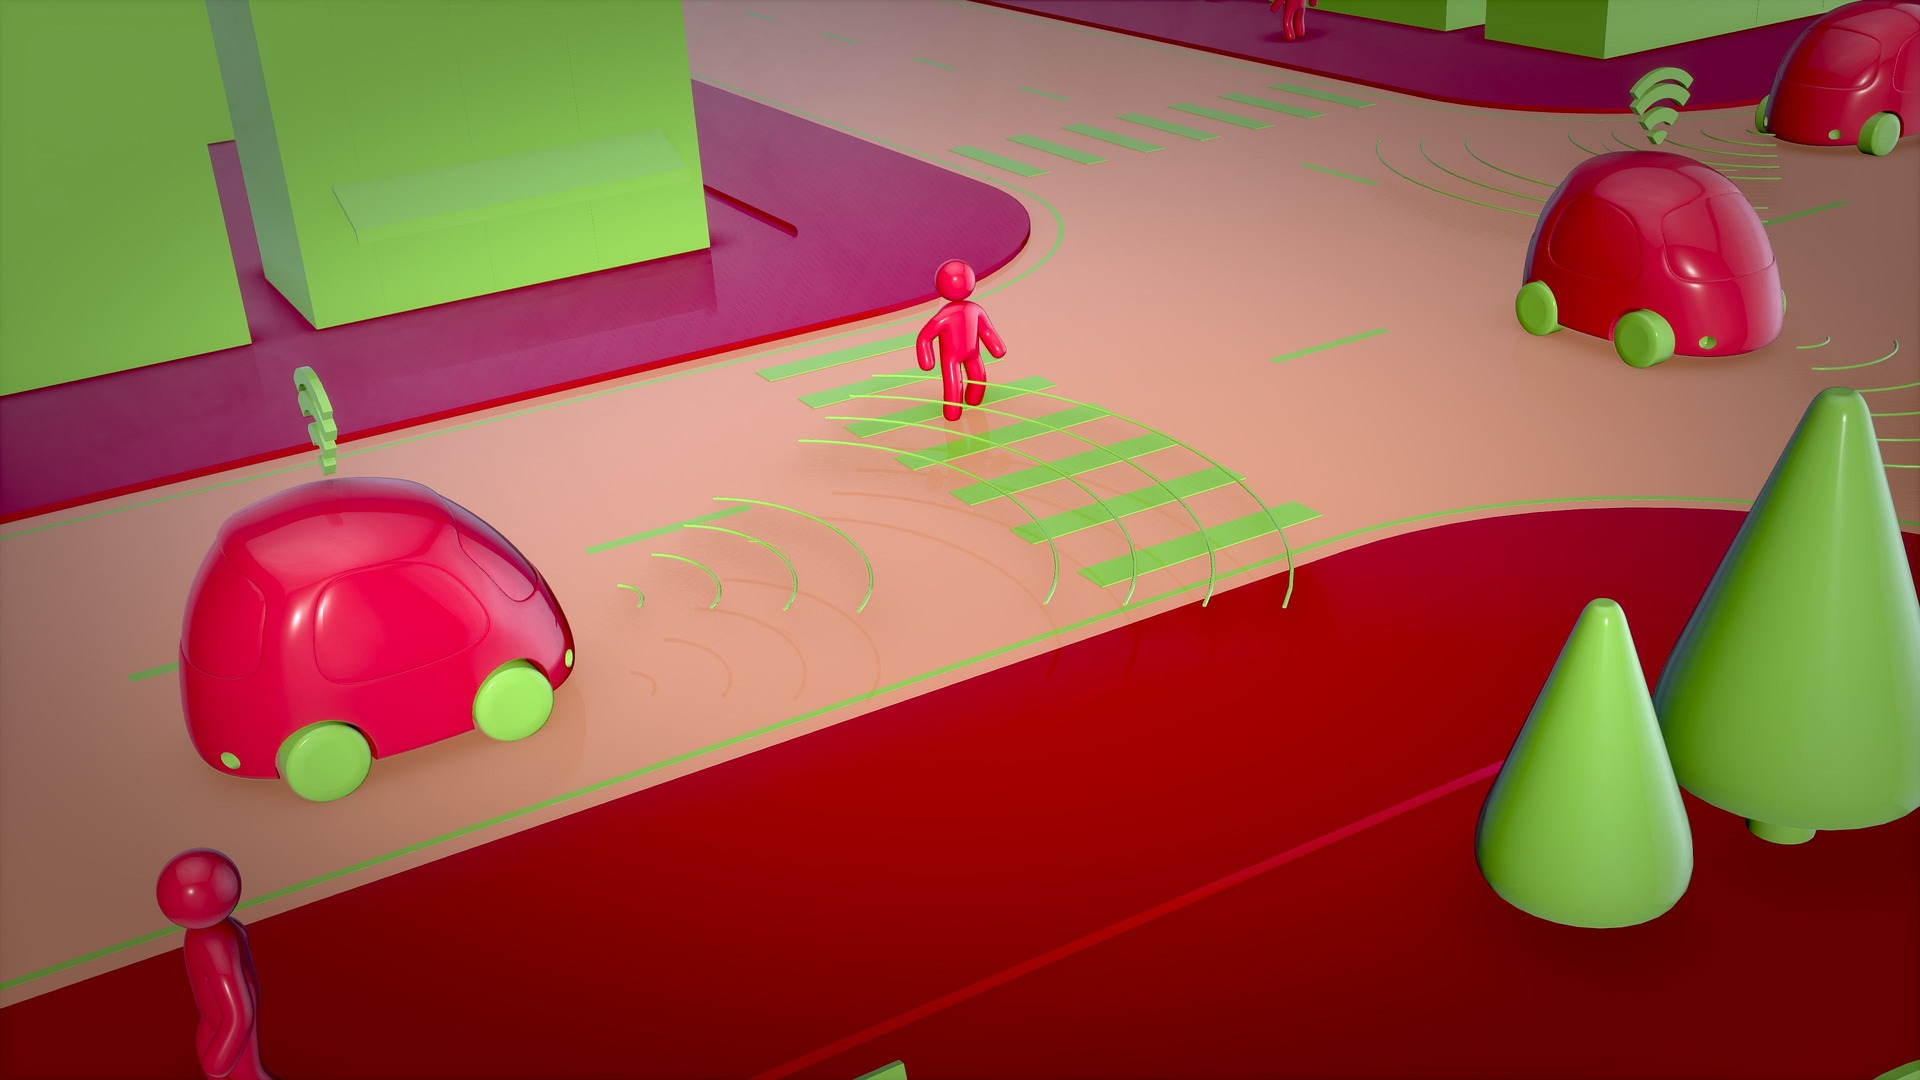
\includegraphics[width=1.0\textwidth]{resources/images/car-4343633_1920.jpg}
        \caption{Autonomes Fahren \cite{car1_img}}
    \end{figure}
\end{frame}

\begin{frame}
    \frametitle{Was ist Autonomes Fahren?}
    
    \begin{itemize}
        \item Fahrzeuge die komplett eigenständig fahren oder den Fahrer unterstützen
        \item In der Fachliteratur werden selbstfahrende Fahrzeuge oft als AVs (autonomous vehicles) bezeichnet
        \item Fahrzeuge sind untereinander und mit der Infrastruktur vernetzt
    \end{itemize}
\end{frame}

\begin{frame}
    \frametitle{SEA-Levels}

    Definiert durch Society of Automotive Engineers \cite{websiteSAE} in Standard J3016 \cite{standardSAE}

    \begin{itemize}
        \item Level 0: Keine Automatisierung
        \item Level 1: Assistenzsysteme
        \item Level 2: Teilautomatisierung
        \item Level 3: Bedingte Automatisierung
        \item Level 4: Hohe Automatisierung
        \item Level 5: Volle Automatisierung
    \end{itemize}
\end{frame}